\documentclass[xcolor=pdftex,dvipsnames,table,mathserif]{beamer}
\usetheme{default}
%\usetheme{Darmstadt}
%\usepackage{times}
%\usefonttheme{structurebold}

\usepackage[english]{babel}
%\usepackage[table]{xcolor}
\usepackage{pgf,pgfarrows,pgfnodes,pgfautomata,pgfheaps}
\usepackage{amsmath,amssymb,setspace,outline}
\usepackage[latin1]{inputenc}
\usepackage[T1]{fontenc}
\usepackage{relsize}
\DeclareMathSizes{10}{10}{6}{6} 


\title{Notes on Numerical Integration}
\author{Chris Conlon  }
\institute{Grad IO}
\date{\today }
\setbeamerfont{equation}{size=\tiny}
\begin{document}

\begin{frame}
\titlepage
\end{frame}


\begin{frame}{Numerical Integration}
We are interested in lots of problems that require computing difficult integrals (e.g.: evaluating expectations )
\begin{enumerate}
\item Midpoint/Trapezoid Rules
\item Simpson's Rule
\item Gaussian Rules
\item Higher-Dimensional Rules
\end{enumerate}
\end{frame}


\begin{frame}{Quadrature Rules}
Basic idea of quadrature is to approximate complicated functions with something easier to integrate, and then integrate that exactly.\\
\begin{figure}[htbp]
\begin{center}
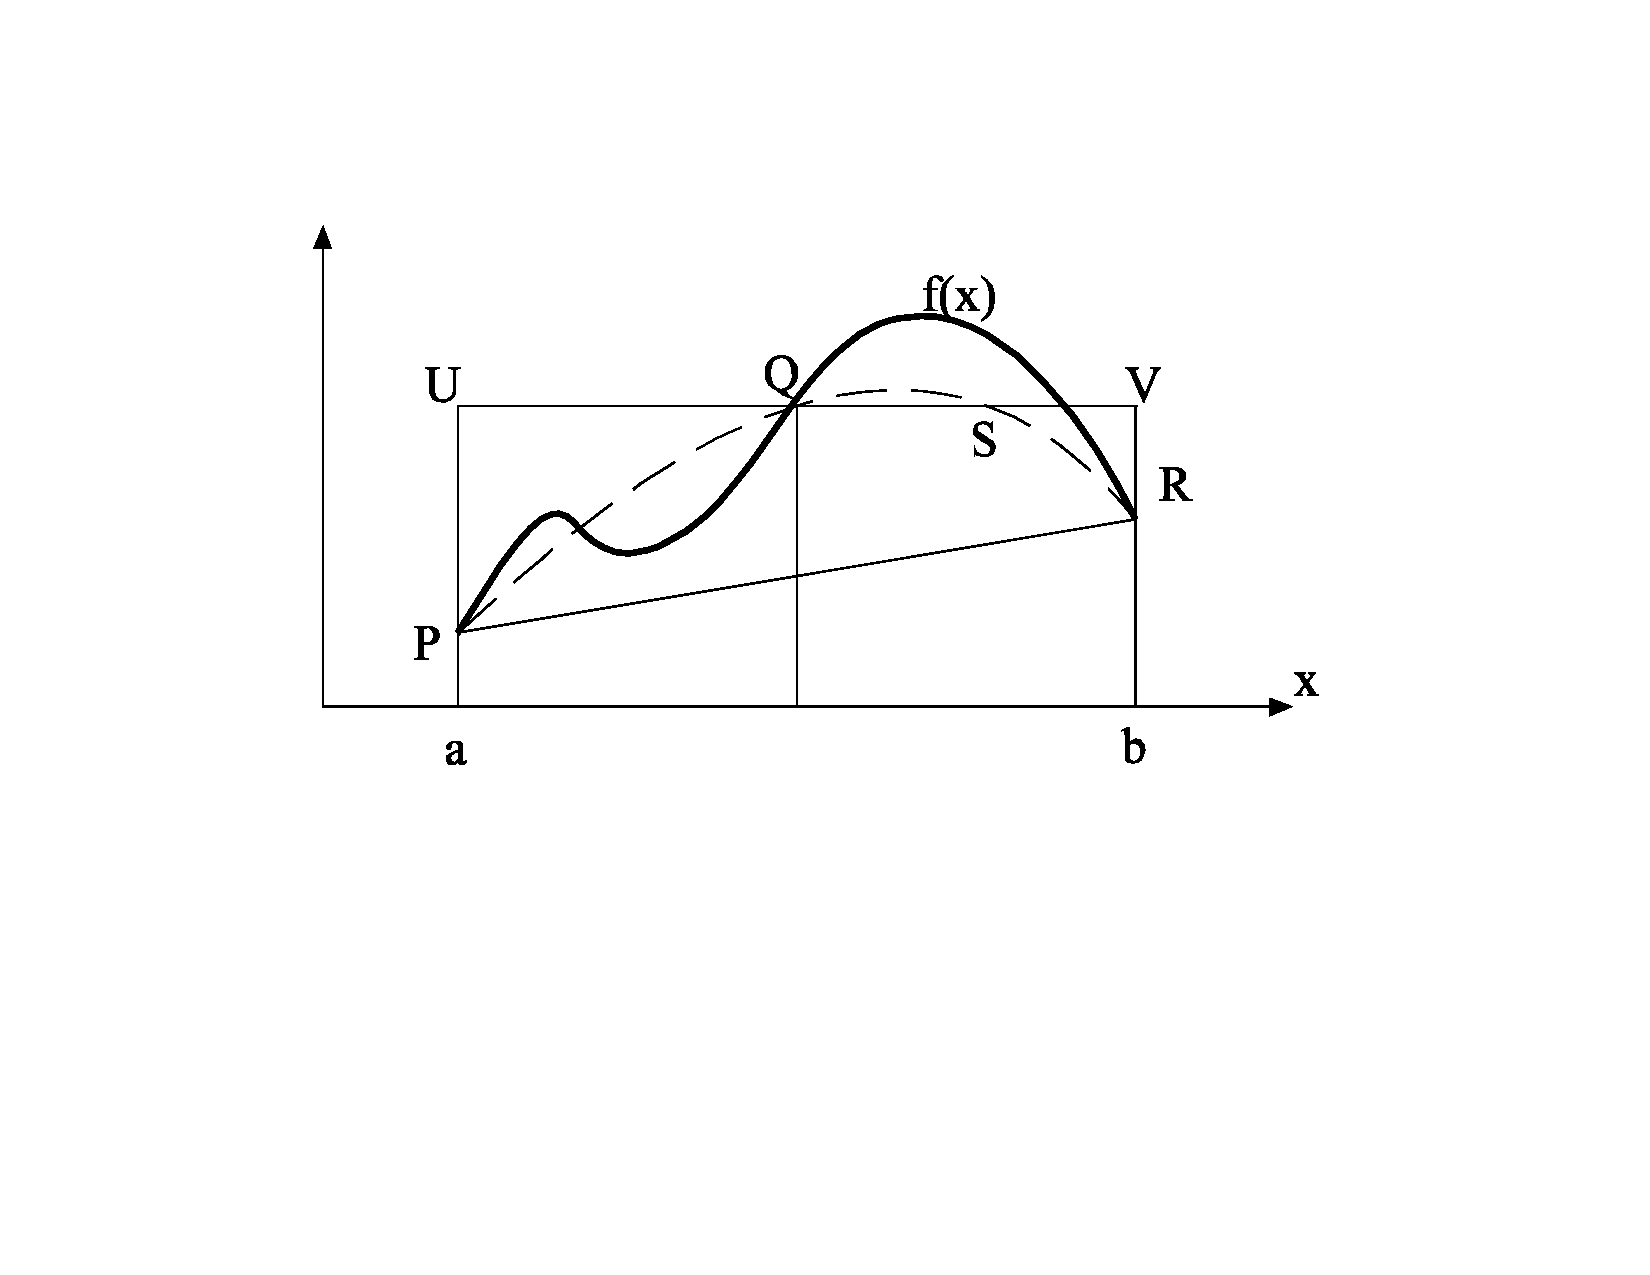
\includegraphics[height=1.75in]{quadrature.pdf}
\end{center}
\end{figure}
\begin{itemize}
\item Constant $f(x)$ at midpoint of $[a,b]$ $aUQVb$ for box.
\item Linear: Trapezoid $a PRb$
\item Parabola through $f(x)$ at $a,b$ and $\frac{a+b}{2}$ for $aPQRb$
\end{itemize}
\end{frame}

\begin{frame}{Simpsons Rule (Newton-Cotes)}
Piecewise Quadratic Approximation at some $\xi \in[a,b]$
\begin{eqnarray*}
\int_{a}^b f(x) d x \approx \left(\frac{b-a}{6} \right) \left[f(a) + 4f \left( \frac{a+b}{2} \right) + f(b) \right]  - \frac{(b-a)^5}{2880} f^{(4)} (\xi)
\end{eqnarray*}
With approximation error
\begin{eqnarray*}
\frac{1}{90} \left( \frac{b-a}{2}\right)^5 | f^{(4)} (\xi) |
\end{eqnarray*}
Works well when quadratic approximation is good $f^{(4)}$ is small or interval is small.
\end{frame}

\begin{frame}{Gaussian Quadrature}
Formulas of the form
\begin{eqnarray*}
\int_{a}^b f(x) d x \approx \sum_{i=1}^n  w_i f(x_i)
\end{eqnarray*}
for some quadrature nodes $x_i \in [a,b]$ and weights $w_i$.
\begin{itemize}
\item Let $\mathcal{F}_k$ be the space of degree $k$ polynomials
\item Quadrature formulas are exact of degree $k$ if it correctly integrates each function in $\mathcal{F}_k$
\item Gaussian quadrature formulas use $n$ points and are exact of degree $2n-1$.
\end{itemize}
Approximation Error
\begin{eqnarray*}
(f,g) = \int_a^b w(x) f(x)  dx - \sum_{i=1}^n w_i f(x_i) = \frac{f^{(2n)}(\xi)}{(2n)!} (p_n,p_n) 
\end{eqnarray*}
\end{frame}

\begin{frame}{Gaussian Quadrature}
\begin{description}
\item[Legendre] Domain: $[-1,1]$, $w(x) = 1$
\item[Chebyshev] Domain: $[-1,1]$, $w(x) = \frac{1}{\sqrt{1-x^2}}$
\item[Laguerre] Domain: $[0,\infty]$, $w(x) = \exp[-x]$ (useful for present value)
\item[Hermite] Domain: $[-\infty,\infty]$, $w(x) = \exp[-x^2]$ (useful for normal)
\end{description}
Helpful if function is $C^{\infty}$ or analytic.
\end{frame}

\begin{frame}{Gauss Herrmite}
Let $Y\sim N(\mu,\sigma^2)$ and apply COV $x = (y-\mu)/\sqrt{2} \sigma$
\begin{eqnarray*}
E[f(Y)] = (2 \pi \sigma^2)^{-\frac{1}{2}} \int_{-\infty}^{\infty} f(y) \exp\left[-\frac{(y-\mu)^2}{2\sigma^2} \right] dy \\
\int_{-\infty}^{\infty} f(y) \exp\left[-\frac{(y-\mu)^2}{2\sigma^2} \right] dy = \int_{-\infty}^{\infty} f(\sqrt{2} \sigma x + \mu) e^{-x^2} \sqrt{2} \sigma dx
\end{eqnarray*}
Gives the quadrature formula using Gauss Hermite $(x_i,w_i)$.
\begin{eqnarray*}
E[f(Y)] = \frac{1}{\sqrt{\pi}} \sum_{i=1}^n w_i f(\sqrt{2}\sigma x_i + \mu)
\end{eqnarray*}
\end{frame}

\begin{frame}{Higher Dimensional Integration}
\begin{itemize}
\item In higher dimension we can use product rules of 1-D integrals.
\item This grows exponentially in dimension $D$ (Curse of Dimensionality)
\item Monte Carlo is not cused but slow to converge $\frac{1}{\sqrt{n}}$ vs $\frac{1}{2n!} f^{(2n)}$
\item Some monomial rules (Judd), (Skrainka and Judd) aren't cursed
\item Sparse Grids show how to combine 1-D rules more efficiently (www.sparse-grids.de)
\end{itemize}
\end{frame}



\end{document}